\documentclass{article}
\usepackage[utf8]{inputenc}

% Used in the explanation text
\usepackage[colorlinks]{hyperref}
\usepackage{graphicx}
\usepackage{tabulary}

% Used by the template
\usepackage{setspace}
\usepackage{changepage} % to adjust margins
\usepackage[breakable]{tcolorbox}
\usepackage{float} % for tables inside tcolorbox https://tex.stackexchange.com/a/274342
\usepackage{enumitem}
\usepackage{geometry}
\geometry{a4paper, portrait, margin=2in, top = 10mm, bottom = 5mm}
\usepackage{caption}



\begin{document}


\newenvironment{mcsection}[1]
    {%
        \textbf{#1}

        % Reduce margins to use the space more effectively and help fit in the recommended "one to two pages"
        % Use the bullet list format as shown in the model card paper to increase readability
        \begin{itemize}[leftmargin=*,topsep=-4pt,itemsep=-1ex,partopsep=1ex,parsep=1ex,after=\vspace{\medskipamount}]
    }
    {%
        \end{itemize}
    }

% Optional: reduce margins single line to fit in "one to two pages", as recommended
\begin{adjustwidth}{-100pt}{-100pt}
\begin{singlespace}

\tcbset{colback=white!5!white}
\begin{tcolorbox}[title=\textbf{Model Card},
    breakable, sharp corners, boxrule=0.7pt]

% Change to a smaller, but still legible font size to help fit in the recommended "one to two pages"
\small{

\begin{mcsection}{Model Details}
    \item Developed by Kamran Chitsaz and Alireza Razaghi for the IFT6390 first project.
    \item Out of distribution classifier
    \item Model has been developed on 2021-03-10
    \item Using Variational Autoencoder to identify if a sample is coming from a similar distribution as the training dataset or not
\end{mcsection}

\begin{mcsection}{Intended Use}
    \item Intended to be used for detecting if a sample is coming from a similar distribution as the training dataset or not
    \item Particularly intended for investigating if a picture is of a number or not
    \item Not suitable for classifying other types of images such as animals or objects
    \item Should not be used for essential topics such as navigation in smart cars 
\end{mcsection}

\begin{mcsection}{Factors}
    \item The model is trained on the MNIST dataset and it is mostly accurate for images with similar resolution, colour and content.
    \item The model is evaluated on images from MNIST and Fashion MNIST datasets to test the accuracy of identifying in distribution and out of distribution samples
\end{mcsection}

\begin{mcsection}{Metrics}
    \item We calculate the log likelihood of a new sample and by comparing it to a threshold, classify it as Out of Distribution or In distribution. The choice of a threshold depends on the particular application. We have tune the threshold, as same as other model hyper parameters, by validation set. 
    \item The decision threshold is -500

\end{mcsection}

\begin{mcsection}{Training Data}
    \item MNIST, training data split
\end{mcsection}



\begin{mcsection}{Evaluation Data}
    \item MNIST, test data split and Fashion MNIST
    \item We used a combination of two datasets to test our model
\end{mcsection}

\begin{mcsection}{Ethical Considerations}
    \item This project shows that VAE can assign spuriously high likelihood to OoD samples which make them unreliable metrics for OoD detection. This model should not be used for any essential topics
\end{mcsection}

\begin{mcsection}{Caveats and Recommendations}
    \item While the idea of identifying out of distribution sample can be used in vast number of topics, a robust solution is still lacking. By introducing an efficient OoD score for VAEs, we can obtain better performance.
    \item Another application of this approach is preventing to input out of distribution data to models to maintain the performance of the model and ensure the quality of the collected data.
\end{mcsection}

\begin{mcsection}{Quantitative Analyzes}
    \item Histogram of the log likelihood of test samples for (a) VAE traind on Mnist and Fashion-Mnist as OoD, and (b) VAE traind on Fashion-Mnist and Mnist as OoD.
    \centering{
    \begin{tabular}{cc}
      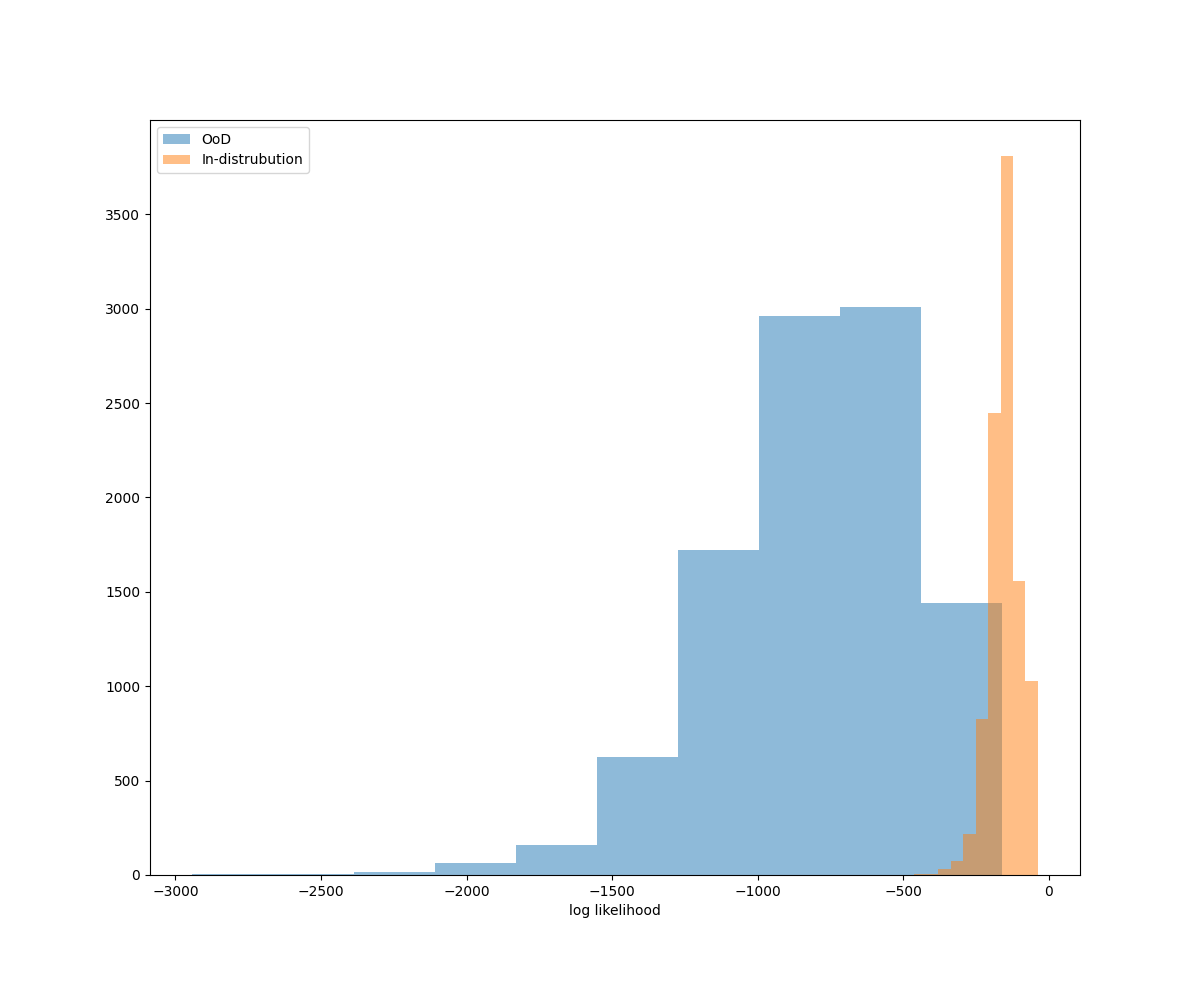
\includegraphics[height=0.24\textheight]{figures/plot_hist.png}
      &
      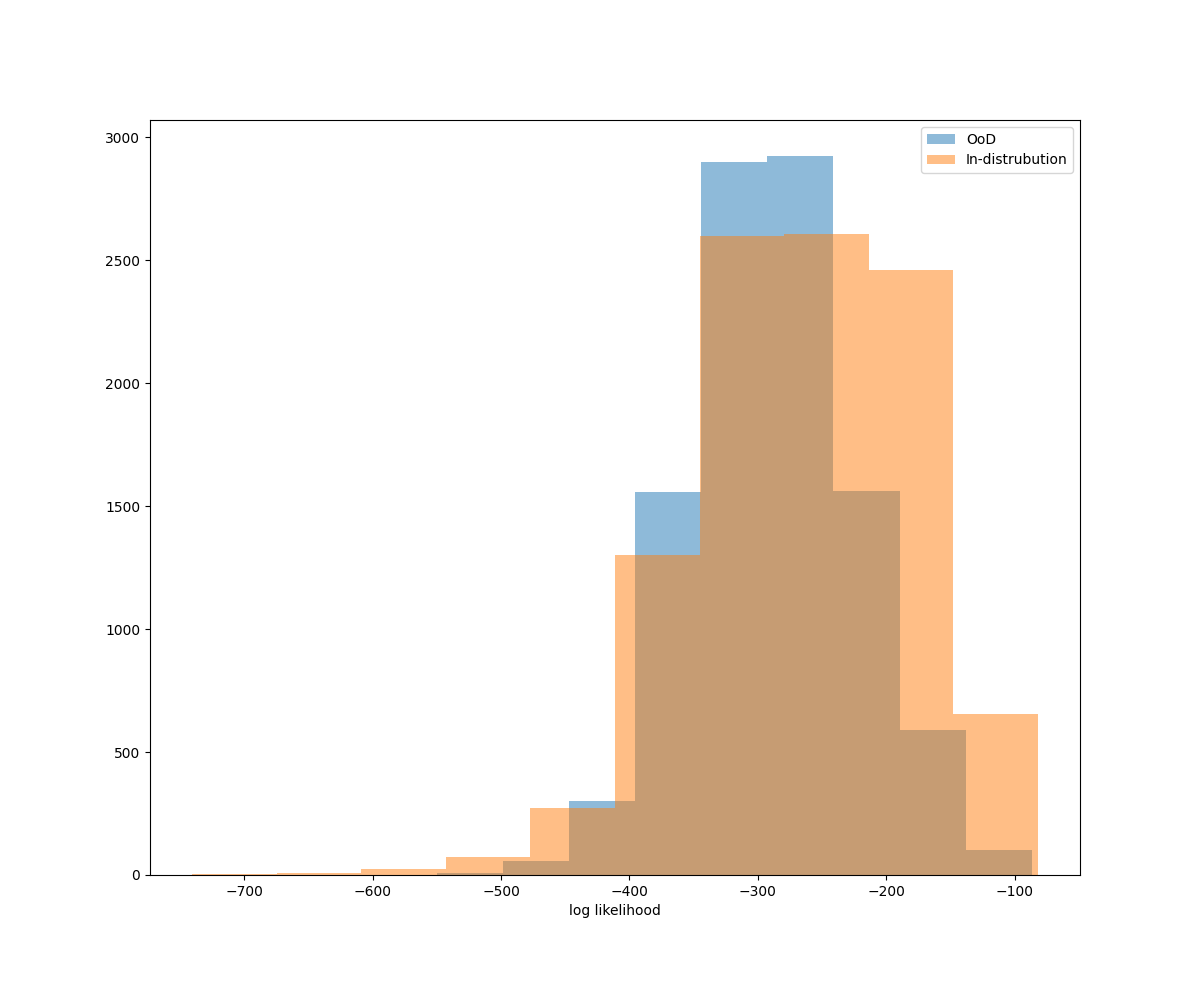
\includegraphics[height=0.24\textheight]{figures/plot_hist_fmnist.png}
       \\                                                     
       a & b
       \end{tabular}
     }
\end{mcsection}


} % end font size change
\end{tcolorbox}
\end{singlespace}
\end{adjustwidth}

\end{document}
